\documentclass[a4paper,12pt]{report}

\usepackage[latin1]{inputenc}		%NOTE: Save File as 'Western (ISO Latin 1)'
\usepackage[T1]{fontenc}
\usepackage[dutch]{babel}

\usepackage{amsmath}
\usepackage{graphicx}			%gif/jpeg/... images
\usepackage{subfigure}
\usepackage{a4wide}				%fullpage
\usepackage{fancyhdr}
\pagestyle{fancy}

%\usepackage{chappg}			%Number pages by chapter

%%%
\usepackage{float}
\floatstyle{boxed}
\newfloat{listing}{h}{lgr}
\floatname{listing}{Listing}
%%%

\begin{document}

\title{
	\textbf{Stageverslag} \\ 
	\normalsize{H04G0A -- Bedrijfservaring: Computerwetenschappen}}
	
	%\includegraphics[scale=.7]{img/cronoslogo}

\author{
	\textbf{Wouter Van Ranst} \\ 
	s0163272, $2^{e}$ Master Computerwetenschappen -- Artifici�le Intelligentie}

\date{1 augustus 2008 -- 9 september 2008}

\maketitle

\tableofcontents

\chapter{Inleiding}
	\section{Administratieve Gegevens}
	
\begin{table}[htbp]
  \begin{tabular}{rl}
    Naam Student: 	& Wouter Van Ranst \\
	Studiejaar: &	$2^{e}$ Master Computerwetenschappen -- Artificiele Intelligentie \\	\\
	Naam Bedrijf:	& Cronos NV, XT-i Extreme Implementations \\
    Adres Bedrijf:	& Veldkant 35A, 2550 Kontich \\
	\\
	Naam Stagebegeleider:	& G�nther Van Roey, Tim Goffings \\
	Stageperiode:	& 1 augustus -- 22 augustus, 3 september -- 9 september 2008
  \end{tabular}
\end{table}
	
	\section{Beschrijving van het bedrijf}
XT-i is een IT servicebedrijf en levert audit, consultancy en projectservices aan klanten uit alle marktsegmenten. Het bedrijf focust op projecten die Java (J2EE) en XML technologie�n integreren. Opgericht in 2001 als deel van de Cronos groep, telt het bedrijf momenteel ongeveer 50 werknemers. Cronos stelt in totaal, over alle deelbedrijven, ongeveer 1250 mensen tewerk.

\chapter{Verslag}
	\section{Probleemstelling}
De Vlaamse krant Het Laatste Nieuws\footnote{http://www.hln.be/}, wil zich in de toekomst meer toespitsen op regionaal nieuws. De krant wil de huidige 5 edities (Antwerpen, Limburg, West-Vlaanderen, Oost-Vlaanderen en Vlaams-Brabant) nog verder opdelen.

De belangrijkste problemen die hierbij moeten worden opgelost zijn het opstellen van de layout (het plaatsen van de artikels op de pagina's) en het snel genoeg kunnen drukken van deze verschillende edities.

Het laatste probleem is opgelost met digitale drukpersen waarbij het manueel verwisselen van drukplaten niet meer nodig is. Het eerste probleem blijft echter.

Momenteel gebeurt het layouten manueel en neemt per editie ongeveer 5 uur in beslag. Als de eerste krant om 05h00 bezorgd moet worden, het drukken 4 uur duurt en het layouten 5 uur, dan kan het laatste artikel ten laatste om 8 uur 'savonds binnenkomen om de krant van de volgende dag te halen. Dit is verre van ideaal.
\\ 
\\
De informatica-afdeling van HLN heeft een eerste layoutalgoritme ontworpen dat binnen 2 uur bruikbare layouts genereert. De bedoeling is met een onbevangen geest (geen informatie over de werking van het huidige algoritme werd gegeven) een nieuw algoritme te ontwerpen dat voldoet aan de gegeven eisen (constraints, zie later) maar binnen een kortere tijdsspanne aanvaardbare layouts genereert.


	\section{Voorstellen}
		\subsection{Fysiek layoutprobleem}
Het vak \textit{Fysieke Logistiek}\footnote{H01R9A, 3e Bachelor Bedrijfsbeheer, Pintelon L.} bespreekt enkele layoutalgoritmes (CRAFT, ALDEP, CORELAP, ...) voor fabrieksplattegronden. Deze plannen voornamelijk oppervlakte met onderlinge afstand (adjacency) als constraint.

Onderlinge afstand is irrelevant voor artikels en de constraint dat geplande `ruimtes' rechthoeken moeten zijn mankeert.

		\subsection{Lineair Programma}
Een lineair programma optimaliseert een lineaire objectieffunctie onderhevig aan (on)-gelijkheidsconstraints.

De objectieffunctie zou bijvoorbeeld de totale oppervlakte witruimte kunnen zijn, maar wegens lineariteit zijn veel kleine witruimtes even slecht dan een grote witruimte (volgens de objectieffunctie). Een grote witruimte die juist te klein is om een artikel in te plaatsen is echter (visueel) veel erger dan meer fragmentaire witruimte.

De totale  prioriteit (belangrijkheid) van de geplaatste artikels maximaliseren is een andere objectieffunctie:
\begin{eqnarray*}
	&max \sum_{i=1}^{n}{ArtikelGeplaatst_i \cdot PrioriteitArtikel_i} \\
	& ArtikelGeplaatst_i = [0,1]
\end{eqnarray*}

De verscheidene constrains die verder in het verslag aan bod komen kunnen vertaald worden naar lineaire constraints.
\\
\\
Een LP-solver is echter een generische solver voor een heel armada van problemen. Fijne controle om het zoekproces te leiden is niet mogelijk, maar er bestaat wel een andere soort constraint programming waar fijne controle wel mogelijk is.

		\subsection{Prolog en varianten}
In het vak \textit{Advanced Programming Languages for A.I.}\footnote{H02A8A, 1e Master AI, Janssens G.} komen enkele moderne constraint solvers aan bod, gebouwd bovenop Prolog.

De ingebouwde backtracking van Prolog maakt het heel geschikt voor een layoutalgoritme. Verschillende layouts kunnen gegenereerd worden d.m.v. backtracking zonder een grote overheadkost.
			
			\subsubsection{CHR}
CHR (Constraint Handling Rules\footnote{http://www.cs.kuleuven.be/$\sim$dtai/projects/CHR/}) laat toe om business rules expliciet neer te schrijven. In het prakticum van voorgenoemd vak bleek dat CHR niet altijd even snel is in vergelijking met pure Prolog, zoals bleek uit het project van eerder genoemd vak.
			
			\subsubsection{ECLiPSe}
ECLiPSe\footnote{http://eclipse-clp.org/} is een constraint logic programming (CLP) systeem dat gebouwd is bovenop Prolog. Het biedt een aantal extra libraries aan die o.m. het adresseren van lijsten (een klassiek pijnpunt in Prolog) gemakkelijker maakt, heuristische zoekfuncties aanbiedt en integer programming mogelijk maakt.
		
		\subsection{Java}
Java is een all-round, objectgeorienteerde programmeertaal waarin bijna alles gemaakt kan worden. Het is een hogere programeertaal die at runtime ge�nterpreteerd wordt. Hierdoor is er veel meer overhead dan nodig voor dit \textit{eenvoudige} probleem.

Java biedt een enorme flexibiliteit, wat hier niet echt nodig is en biedt geen ingebouwde backtracking, wat hier wel nodig is.

		\subsection{Conclusie}
Java valt uit de boot door te veel overhead en de fysieke layoutalgoritmes zijn onaangepast. Van de Prolog varianten is CHR de traagste. ECLiPSe lijkt, mede door zijn opzet, de geknipte kandidaat voor het probleem op te lossen.

	\section{Invoer}
De door de journalisten geschreven artikels worden door QuarkXPress gerenderd tot verschillende mogelijke vormen (verschillende hoogte/breedte, andere kop, ander lettertype, ...). Dit resulteert in een reeks `rechthoeken'. Samen met de grootte van elke pagina en eventuele ruimte voor advertenties wordt dit geexporteerd naar XML. Een ingekorte versie van een dergelijk XML bestand staat in listing \ref{listing:inXML} (pagina \pageref{listing:inXML} e.v.). Het XML bestand bevat 4 (lege) pagina's, pagina 2 bevat een advertentie. In totaal zijn er 66 artikels, waarvan 6 kopstukken, 29 normale en 31 korte artikels.

			\subsubsection{Pagina's}
De belangrijkste gegevens van de \verb|page| nodes, zijn \verb|usewidth| en \verb|useheight|. Dit zijn respectievelijk de bruikbare breedte en hoogte van de pagina. Merk op dat dit kan verschillen van pagina tot pagina. Verder is er ook het \verb|id| van de pagina, een uniek nummer per pagina.

			\subsubsection{Artikels}
De belangrijkste gegevens van de \verb|artikel| nodes, zijn \verb|type|, \verb|plaatsing|. De belangrijkste gegevens van de \verb|artlayout| subnodes, zijn \verb|width|, \verb|height|.

\paragraph{Type} Er zijn 3 types. \verb|Kopstuk| betekent dat het artikel enkel geplaatst mag worden tegen de bovenkant. \verb|Normaal| betekent een normaal artikel en \verb|Kortje| betekent een klein artikel (merk op het verschil in width en height), typisch met maar 1 layoutmogelijkheid.

\paragraph{Plaatsing} Er zijn 3 plaatsingsmogelijkheden. Een artikel met een plaatsing \verb|V| moet \textit{vooraan} in de regionale sectie geplaatst worden. Een artikel met plaatsing \verb|M| in het \textit{midden} en een artikel met plaatsing \verb|A| \textit{achteraan}.

\paragraph{Artlayout} Een artikel heeft ��n of meerdere layouts. Elke layout heeft een uniek (over alle artikels) nummer \verb|id| dat de layout identificeert, een \verb|width| en een \verb|height|, dewelke de afmetingen van de rechthoek waarbinnen het artikel geplaatst zal worden, bepalen.

	\section{Algoritme 1}
		\subsection{Algoritme}
Elke pagina wordt gediscretiseerd in een paar rijen en kolommen. Voor elk artikel wordt berekend hoeveel rijen en kolommen het zal innemen. 
\begin{enumerate}
	\item Kies het te plaatsen artikel. Dit is hier eenvoudigweg in volgorde van het invoerbestand. 
	\item Kies een layout van het artikel. Dit is hier eenvoudigweg in volgorde van het invoerbestand.
	\item Zoek op de pagina een vrije ruimte waar het artikel met de layout (met bepaalde afmetingen) geplaatst kan worden, rekening houdend met plaatsingsregels\footnote{Bijvoorbeeld: Kopstukken mogen enkel op de eerste rij geplaatst worden. Dit is de enige geimplementeerde regel.}. Indien er geen ruimte is, ga naar het volgende artikel (stap 1).
	\item Wijs de ruimte op de pagina toe aan het artikel. Ga naar het volgende artikel (stap 1).
\end{enumerate}
			
		\subsection{Implementatie}
\paragraph{Geheugenstructuur toegewezen artikels} De gediscretiseerde pagina (met aantal kolommen C en aantal rijen R) wordt in het geheugen bijgehouden als een CxR matrix. De elementen van de matrix zijn op dit ogenblik vrije variabelen. Bij de toewijzing van een artikel aan de pagina krijgen de elementen die binnen de rechthoek vallen de waarde van het artikel id. De representatie in het geheugen heeft dus een visuele betekenis. Als de matrix wordt uitgeprint is de layout zichtbaar. Een voorbeeld staat in listing \ref{listing:layouteersteopl}.

\paragraph{Zoek vrije ruimte} Het zoeken van een vrije ruimte op de pagina begint bij een startcoordinaat (hier (1,1) van de discrete pagina). Bereken de afmetingen van de rechthoek. Controleer of er overlap is met een ander, eerder geplaatst artikel. Indien er geen overlap is mag het artikel daar geplaatst worden. Indien er wel overlap is, probeer dan de volgende coordinaat. De matrix wordt doorlopen van links naar rechts, en van boven naar onder.
			
		\subsection{Uitvoering}
Met een grid van 10x15 wordt na 0,01s\footnote{Apple MacBook, Intel Core 2 Duo 2,16 GHz, 3 GB RAM, OS X Leopard 10.5.4, ECLiPSe 5.10} de eerste oplossing uitgeprint. De stappen dat het algoritme uitprint zijn weergegeven in listing \ref{listing:opeenvolgendegeplaatsteartikels} (pagina \pageref{listing:opeenvolgendegeplaatsteartikels}). De gegenereerde layout is weergegeven in listing \ref{listing:layouteersteopl}. De volgende oplossing, berekend na 0,05s meer, verschuift het laatst geplaatste artikel (met id 30902) ��n eenheid naar rechts. De gegenereerde layout is weergegeven in listing \ref{listing:volgendeopl}.
\\
\\
Onderstaande tabel toont voor verschillende dimensies de tijd tot het berekenen van respectievelijk de eerste, tweede en zestigste oplossing.
      
\begin{table}[h]
  \centering
  \begin{tabular}{c|cccc}
	Dimensie (BxH) & 1e Opl. & 2e Opl. & & 60e Opl. \\
	\hline
    10x15 & 0,01s & 0,06s & & 0,75s \\ 
    20x30 & 0,03s & 0,06s & $\ldots$ & 1,63s \\ 
    80x120 & 0,22s & 0,42s & & 11,48s \\ 
  \end{tabular}
  \caption{Uitvoeringstijden voor verschillende dimensies}
  \label{tab:exectimesalg1}
\end{table}
				
		\subsection{Conclusie}
Dit algoritme genereert voor de gegeven artikels elke mogelijke layout, ongeacht of deze esthetisch aanvaardbaar is of niet. Een goede layout zal naar alle waarschijnlijkheid pas laat in het zoekproces tevoorschijn komen. Om een goede bladvulling te bekomen moet ook het discretisatiegrid groot genoeg gedimensioneerd worden (de afmetingen van artikels worden naar boven afgerond en zal er bij een klein grid dus veel \textit{verloren} ruimte zijn). Er moeten dus veel layouts op een groot grid berekend worden. Zoals de laatste rij van tabel \ref{tab:exectimesalg1} laat zien kan dit onaanvaardbaar lang duren. 

In het voorbeeld van listing \ref{listing:opeenvolgendegeplaatsteartikels} worden 5 artikels geplaatst op een 10x15 grid. De orde van het aantal plaatsingsmogelijkheden\footnote{Aantal plaatsingsmogelijkheden per artikel: $(GridWidth-ArtWidth+1) \cdot (GridHeight-ArtHeight+1)+1$, Toegepast op voorbeeld: $29 \cdot 53 \cdot 92 \cdot 118 \cdot 118 \approx 2\cdot10^{9}$} is $10^{9}$. Gezien de tijd om 60 mogelijkheden te berekenen, zal het berekenen van deze mogelijkheden orde 100 dagen duren.

De oorzaak hiervoor is de geheugenstructuur voor toegewezen artikels, en het zoeken naar vrije ruimte om een artikel te plaatsen, dewelke op inefficiente wijze gebeuren.

	\section{Algoritme 2}
Het voorgaande algoritme kan op verscheidene punten verbeterd worden.
\begin{enumerate}
	\item \textit{Verloren} ruimte door (te) klein grid (discretisatiefout); \label{VerlorenRuimte}
	\item Zoeken naar vrije ruimte, keuze van beginpunt; \label{ZoekenVrijeRuimte}
	\item Geheugenstructuur geplaatste artikels; \label{Geheugenstructuur}
	\item Keuze van te plaatsen artikel; \label{KeuzePlaatsArtikel}
	\item Intelligent zoeken naar een esthetische layout. \label{Heuristiek}
\end{enumerate}

		\subsection{Idee}
Artikels beginnen niet willekeurig op een pagina. Artikels beginnen in een hoek van de pagina of aan de hoek van een ander artikel. Dit zorgt voor een layout waar inherent al weinig whitespace overblijft en een drastisch kleinere zoekruimte (probleem \ref{ZoekenVrijeRuimte}). Deze benadering pakt ook probleem \ref{VerlorenRuimte} aan doordat niet langer op een discreet grid gewerkt wordt.

Het defini�ren van een heuristische functie die een score aan een bepaalde layout geeft. Een zoekmethode kan zo zoeken naar een \textit{goede} layout (problemen \ref{KeuzePlaatsArtikel} en \ref{Heuristiek}).

			\subsubsection{Heuristiek}
De heuristiek kent een grote score toe aan artikels die goed passen in de al bestaande layout. De heuristische waarde van een plaatsing is (bij benadering) gelijk aan de lengte van de zijden van het artikel die tegen een ander artikel of paginarand liggen. Figuur \ref{fig:inpassingsheur} verduidelijkt het idee.

\begin{figure}[h]
	\centering
	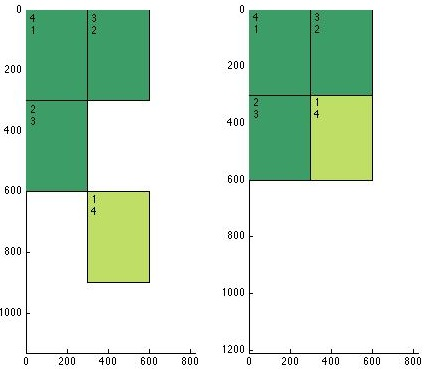
\includegraphics[width=5 cm]{img/inpassingsheur}
	\caption{Twee mogelijke plaatsingen van het lichtgroene artikel. Links een slechte, rechts een goede volgens de inpassingsheuristiek.}
	\label{fig:inpassingsheur}
\end{figure}

Een grote zijde die inpast is beter dan twee kleinere zijden die in totaal even groot zijn. Een (kleine) machtsverheffing zorgt ervoor dat de grote zijde hier de overhand krijgt\footnote{$4^{1,2} > 2^{1,2} + 2^{1,2}$}.

Een zijde die exact even groot is dan de aanliggende zijde is esthetisch ook mooier. Een factor (bovenop de machtsverheffing) zorgt hier voor een grotere score.

		\subsection{Algoritme} \label{subsection:algoritme2algoritme}
De pagina is een rechthoek met een bepaalde breedte en hoogte. Artikels zijn rechthoeken met een bepaalde breedte en hoogte en hebben meerdere layouts.

Artikels worden aangehecht aan een \textit{ankerpunt}. Een artikel kan aan een ankerpunt worden aangehecht op 4 mogelijke manieren: rechtsonder, rechtsboven, linksonder, linksboven.

\begin{figure}[h]
	\centering
	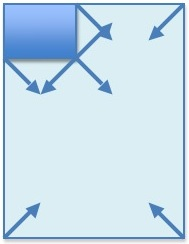
\includegraphics[width=3 cm]{img/ankerpunten}
	\caption{Een pagina met 1 artikel, de 6 ankerpunten met elk de mogelijke richtingen.}
	%\label{fig:vb}
\end{figure}

\paragraph{Opmerking over de gebruikte zoekmethode} In de volgende beschrijving wordt er Greedy Search\footnote{Best first} gebruikt. Andere zoekmethodes zijn ook mogelijk, zoals complete search of optimal search (A*), mits een goede schattingsfunctie voor de uiteindelijke layout op basis van de (reeds gevonden) parti�le layout gevonden kan worden.  \\

De stappen die worden doorlopen zijn:
\begin{enumerate}
	\item[] Start met lege paginas. Lege paginas hebben 4 ankerpunten: de 4 hoekpunten. Voeg eventuele advertenties toe per pagina. Advertenties hebben geen ankerpunten\footnote{Om te vermijden dat het eerste artikel niet linksboven tegen de rand, maar tegen de advertentie wordt geplaatst.}.
	\item Zoek het artikel met de hoogste heuristische score. \textit{In het geval van het eerste artikel op de pagina wordt het grootste artikel geplaatst omdat dit de grootste inpassing kan realiseren.}
	
	\begin{enumerate}
		\item Kies een (mogelijk) artikel.
		\item Kies een (mogelijke) pagina.
		\item Kies een (mogelijke) layout van het artikel die past op de pagina.
		\item Kies een (mogelijk) ankerpunt van de pagina.
		\item Kies een (mogelijke) richting van het ankerpunt waarbij de plaatsing van het artikel volledig op de pagina kan en waar geen overlappig gebeurt met andere artikels.
		\item Contoleer of de huidige plaatsing overeenkomt met de business rules. Geimplementeerd zijn:
			\begin{itemize}
				\item Kopstukken beginnen enkel tegen de bovenste paginarand.
				\item Artikels met voorkeursplaatsing vooraan mogen niet op de achterste pagina geplaatst worden. Artikels met voorkeursplaatsing achteraan mogen niet op de voorste pagina geplaatst worden.
			\end{itemize}
		\item Bereken de score van deze plaatsing volgens de heuristiek.
		\item Overloop de volgende mogelijkheden: een ander(e) mogelijk(e) richting, ankerpunt, layout, pagina, artikel.
	\end{enumerate}
	
	\item Plaats het gevonden artikel (op de in stap 1 bepaalde pagina, layout, ankerpunt en richting). Genereer 4 nieuwe ankerpunten (de 4 hoekpunten van het artikel) en voeg deze toe aan de lijst ankerpunten pagina.
	
	\item Ga naar stap 1.
\end{enumerate}

\begin{figure}[h!]
	\centering
	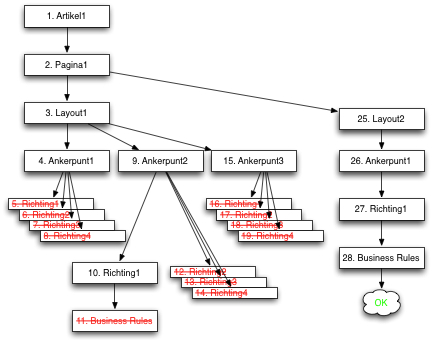
\includegraphics[width=0.76\textwidth]{img/backtracking}
	\caption{De zoekboom van algoritme 2. De cijfers geven de volgorde stappen van het algoritme aan.}
	\label{fig:zoekboom}
\end{figure}

		\subsection{Implementatie}
\paragraph{Geheugenstructuur toegewezen artikels} Probleem \ref{Geheugenstructuur} is het enige dat nog niet besproken. Door de toegewezen artikels bij te houden in een lijst neemt het geheugengebruik hiermee lineair toe.
		
		\subsection{Uitvoering}
Het resultaat van dit algoritme met het voorbeeldbestand verkregen van Het Laatste Nieuws als invoer is te zien op figuur \ref{fig:hlnbestfirst}. Het zoekalgoritme is Greedy Search, zoals eerder beschreven, waarvan de uitvoeringstijd 6 seconden bedraagt. Een complete search was na 5 dagen nog steeds bezig.

De uitvoer van het algoritme tijdens de uitvoering is (verkort) weergegeven in listing \ref{listing:uitvoeralg2}.

\begin{figure}[h]
	\centering
	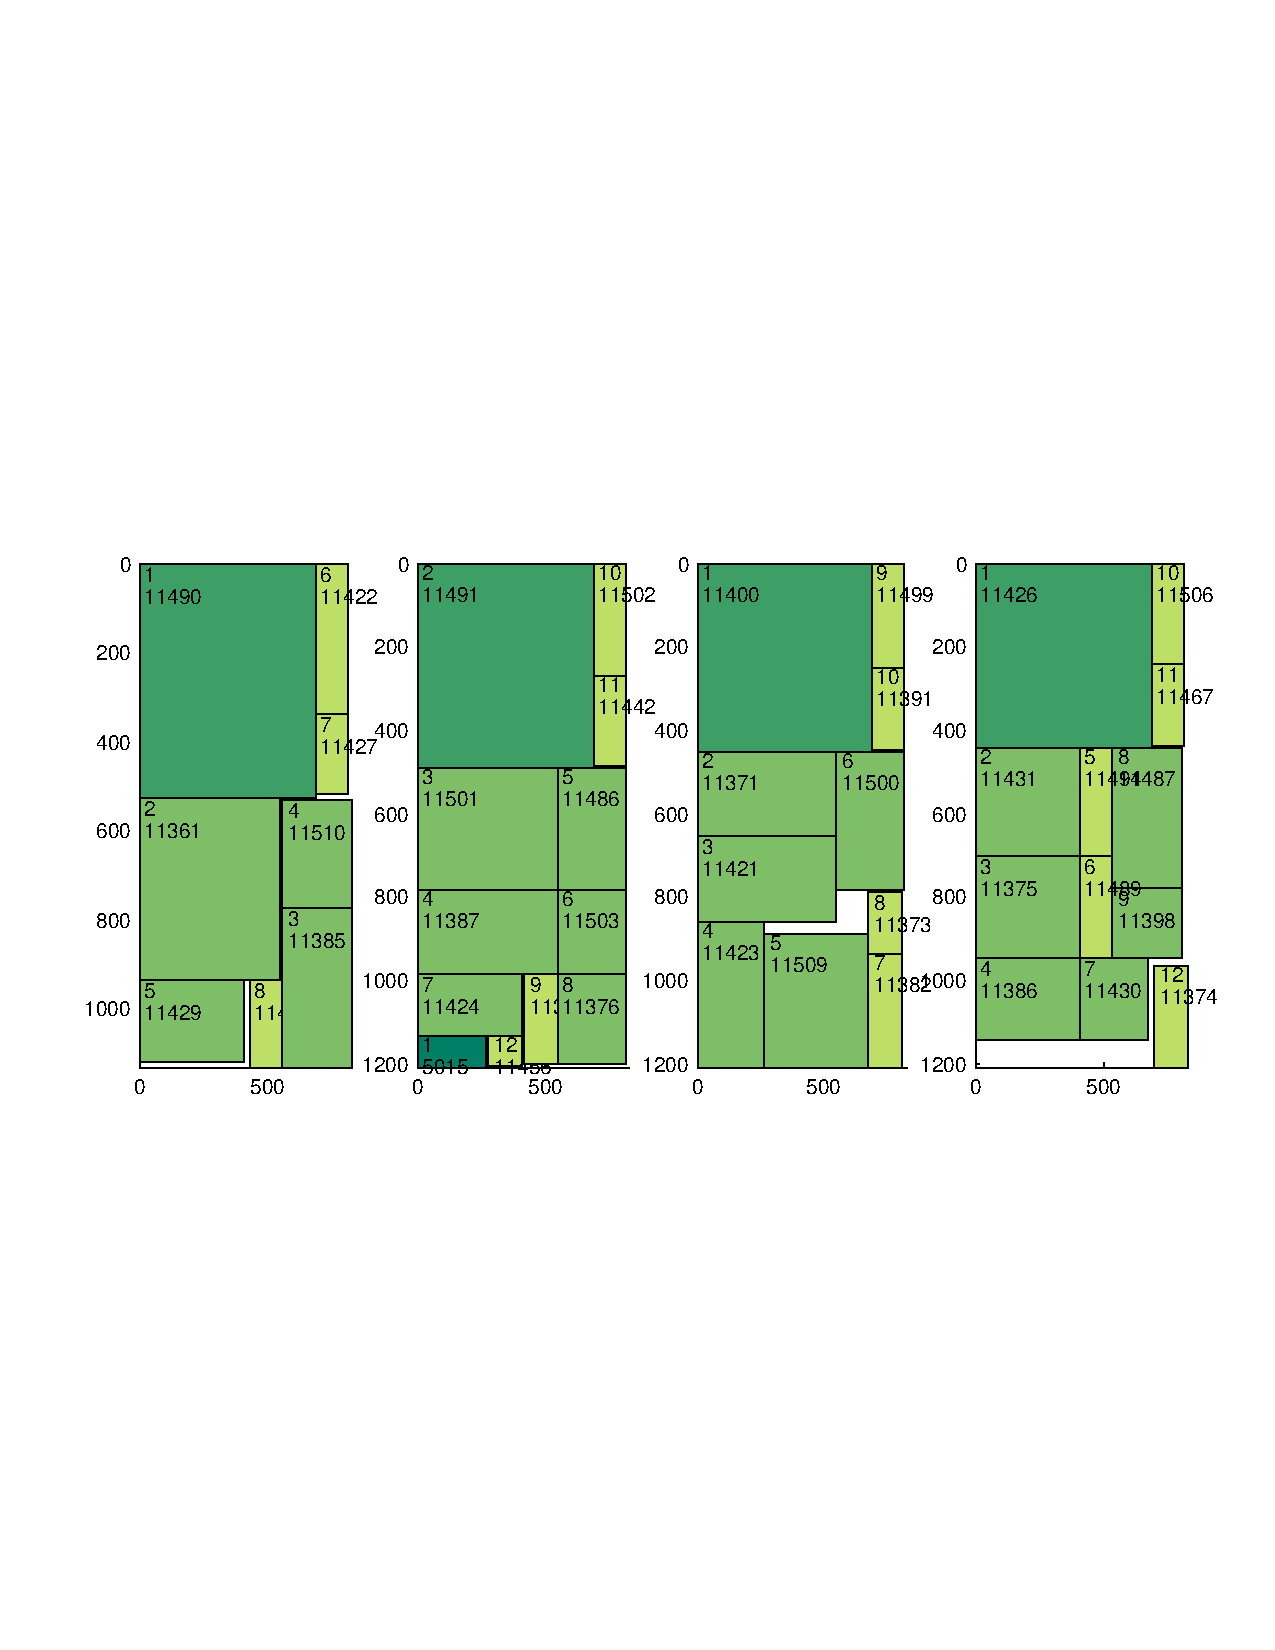
\includegraphics[width=\textwidth, trim=2cm 9cm 1cm 9cm, clip=true]{img/hlnbestfirst.pdf}
	\caption{Resultaat van algoritme 2. Donkergroen: kopstukken, groen: normale artikels, lichtgroen: korte artikels. Het eerste cijfer duidt op de plaatsingsvolgorde op de pagina, het tweede cijfer is het layout id. Bemerk de advertentie linksonder op de tweede pagina (zeer donkergroen) met plaatsingsnummer 1.}
	\label{fig:hlnbestfirst}
\end{figure}

		\subsection{Conclusie}

De uitvoeringstijden en heuristische scores van dit algoritme met de verschillende zoekmethodes zijn weergegeven in tabel \ref{tab:exectimesalg2}. 

Van de Greedy variant zijn er slechts 42 mogelijke oplossingen, de eerste oplossing bevat 41 artikels en elke volgende oplossing bevat een artikel minder.

Van de Complete variant zijn er heel veel\footnote{Grof overschat: 44 plaatsingen kiezen uit 66 artikels  $\cdot$ gemiddeld 2 layouts per artikel $\cdot$ 4 pagina's $\cdot$ 25 ankers per pagina $\cdot$ 4 richtingen per anker $ = C^{52800}_{44} \approx 2E153$ mogelijkheden.} mogelijke oplossingen. De beste oplossing die na 5 dagen rekenen was gevonden had een heuristische score van ongeveer 98000. Bemerk dat dit nog een eind verwijderd is van de score die de Greedy variant na 6 seconden al vindt. Het berekenen van de beste oplossing met complete search\footnote{Met snelheid van $\frac{3,83s}{60 opl} = 6,3E$-2s} zou 1,5E152 seconden duren. Ter vergelijking: het universum bestaat 4,3E17 seconden. Een goede zoekstrategie is dus gerechtvaardigd.

\textit{Hoewel bij beide zoekstrategie�n de heuristische waarde wordt berekend, is dit bij de Complete variant louter informatief. Enkel de Greedy variant gebruikt deze waarde om het zoekproces te sturen.}

Beide eerste oplossingen zijn te zien in figuur \ref{fig:layouts}, pagina \pageref{fig:layouts}. De Greedy variant (figuur \ref{fig:layouts:greedy}) bevoordeelt de indirect grote artikels, omdat deze een grotere inpassing kunnen realiseren. Kleinere artikels komen pas later in het zoekproces aan bod, wanneer de pagina's eventueel al vol staan. 

De Complete variant (figuur \ref{fig:layouts:complete}) plaatst meer en kleinere artikels. De layout is echter chaotisch en er is veel whitespace die weggewerkt zou kunnen worden door te schuiven met de artikels. Grote artikels hebben hier geen voordeel op kleine artikels. Artikels die eerder in het XML bestand staan hebben echter wel voordeel bij deze strategie.

\begin{table}[h]
  \centering
  \begin{tabular}{cc|cccccccc}
	\multicolumn{2}{c}{Methode} & 1e Opl. & 2e Opl. & & 42e Opl. & & 60e Opl. \\
	\hline	
    Greedy & (tijd)	& 6,19s & 6,26s & $\ldots$ & 6,67s & & --  \\ 
    & (score) & 105293.2 & 104955.5 & & 0 \\ \hline
    Complete & (tijd) & 0,69s & 0,88s & $\ldots$ & 2,88s & $\ldots$ & 3,83s & $\ldots$ & 5 dagen\\
     & (score) & 96272.2 &  96272.2 & & 95944.8 & & 96235.8 & & $\sim$98000\\
  \end{tabular}
  \caption{Uitvoeringstijden voor verschillende zoekalgoritmes}
  \label{tab:exectimesalg2}
\end{table}
		
	\subsection{Embedding}
ECLiPSe biedt een embeddable runtime aan die o.a. via een Java ARchive (JAR) aangesproken kan worden.

Het omhullende Java programma leest het XML bestand in en zet dit om naar \mbox{ECLiPSe} structures. Een RPC (Remote Procedure Call) met gepaste query roept het eerder beschreven algoritme aan. De uitvoer verschijnt in de terminal en het resultaat wordt teruggegeven naar het Java programma. Hieruit worden voor elk artikel de paginaId, layoutId, startX en startY gehaald (layoutId en startcoordinaten bepalen een artikel-rechthoek). Deze informatie wordt via een XML DOM parser bij in het invoer XML bestand geschreven. Een ingekorte versie van een dergelijk XML bestand staat in listing \ref{listing:uitvoerxml}. Aan de hand hiervan kan een krantenlayout gegenereerd worden.

	\section{Algoritme 2.1}
Na een bezoek aan de redactie kwamen volgende extra functionele eisen (FR) aan het licht:

\begin{enumerate}
	\item Een pagina heeft mogelijk een gereserveerd kopstuk. Het kopstuk in kwestie moet op die pagina staan. Pagina's zonder gereserveerd kopstuk krijgen een willekeurig kopstuk. \label{gereserveerdkopstuk}
	
	\item Artikels met foto moeten geschrankt geplaatst worden (boven-links, midden-rechts, onder-links, zie figuur \ref{fig:placeholders:ph1}) voor visueel comfort. \label{geschrankteartikels}
	
	\item Artikels die eerder in het XML bestand staan zijn belangrijker en moeten bij voorkeur wel geplaatst worden. \label{arteerderxmlbelangrijker}
	
	\item Bij artikels met meerdere layoutmogelijkheden staat de voorkeurslayout eerst in het XML bestand. \label{layouteerderxmlbelangrijker}
	
	\item Een pagina heeft juist 6 kolommen \label{zeskolommen}.
	
	\item Er mogen niet meer dan twee basislijnen tussen twee artikels staan als open ruimte. \label{tweebasislijnen}
	
	\item Geen twee kaders naast/onder elkaar.
	\item Geen twee foto's naast elkaar.
	\item Geen twee titels met zelfde font en zelfde font size naast elkaar.
\end{enumerate}

De extra gegevens nodig om deze extra FRs te kunnen accommoderen werd in een extra XML bestand aangeleverd.

		\subsection{Idee}
Om tegemoet te komen aan de extra FRs nummer \ref{zeskolommen} en \ref{tweebasislijnen} wordt de pagina opgedeeld in 6 kolommen, elk artikel bezet een veelvoud van een kolom. De hoogte van de artikels wordt ook afgerond op 1 basislijn (de \textit{eenheid} = 9,6 punten).

		\subsection{Algoritme}
\begin{enumerate}
	\item Zet artikels om naar werkbare vorm (afmetingen in $(x \cdot kolombreedte, y \cdot basislijnen)$)
	\item Zet pagina's om naar werkbare vorm
	\item Plaats advertenties
	\item Plaats gereserveerde kopstukken (FR \ref{gereserveerdkopstuk}):
		\subitem Zoek het desbetreffende kopstuk en voer stap 7 uit.
	\item Plaats overige kopstukken:
		\subitem Filter alle overblijvende kopstukken en voer stap 7 uit.
	\item Plaats fotoartikels geschrankt (FR \ref{geschrankteartikels}):
		\subitem Filter alle fotoartikels en voer stap 7 uit.
	\item Plaats overige artikels: zie paragraaf \ref{subsection:algoritme2algoritme}, echter zonder zoekfunctie. Dit garandeert FRs \ref{arteerderxmlbelangrijker} en \ref{layouteerderxmlbelangrijker} doordat het eerste artikel in de lijst ongeplaatste artikels het belangrijkste is, idem voor de layouts van dat artikel. 
	
Als hierover gezocht zou worden (welk artikel met welke layout kan de grootste heuristische waarde realiseren) dan wordt deze FR niet gerespecteerd. Wel zou het mogelijk zijn te zoeken op welk \textit{ankerpunt} van een pagina een layout van een artikel best geplaatst kan worden.

Afhankelijk van het type te plaatsen artikel (fotoartikel of niet) wordt een zijsprong gemaakt om het schranken (FR \ref{geschrankteartikels}) te accomoderen. Bij een niet-fotoartikel wordt de normale flow gevolgd, maar bij een fotoartikel zijn er slechts 2 ankerpunten: onder het eerste kopstuk tegen de rand en in de linkeronderhoek.
\end{enumerate}

		\subsection{Implementatie}
Functionele vereisten 6--9 zijn niet geimplementeerd binnen het gegeven tijdskader.

Het stramien van het vorige algoritme is ruimschoots overgenomen, maar een herimplementatie van het algoritme reduceert de uitvoeringstijd verder.

De eerste oplossing berekenen met algoritme 2 duurt 0,7 seconden\footnote{complete search; geen heuristiek, zoals algoritme 2.1} voor 4 paginas. De eerste oplossing met algoritme 2.1 duurt 0,3 seconden voor 6 paginas, een tijdsreductie van 70\%.

		\subsection{Uitvoer}
Het resultaat van dit algoritme met het (nieuwe) voorbeeldbestand verkregen van Het Laatste Nieuws als invoer is te zien op figuur \ref{fig:alg21uitvoer}. 

\begin{figure}[h]
	\centering
	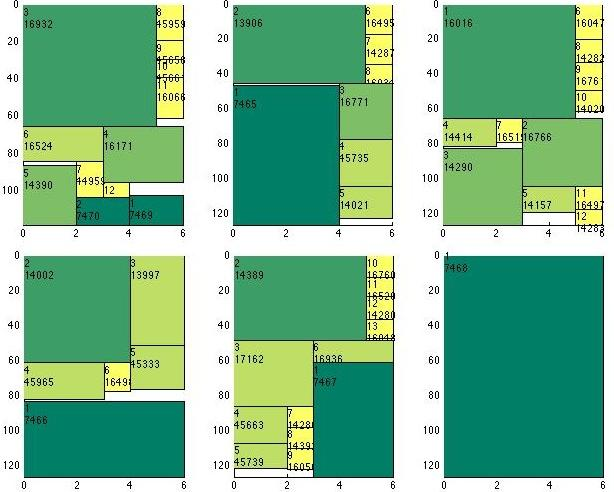
\includegraphics[width=0.8\textwidth]{img/alg21}
	\caption{Resultaat (paginas) van algoritme 2.1. Donkergroen: advertenties, groen: fotoartikels (bemerk geschrankte artikels op pagina 1 en 3), lichtgroen: normale artikels, geel: korte artikels. Het eerste cijfer duidt op de plaatsingsvolgorde op de pagina, het tweede cijfer is het artikel id.}
	\label{fig:alg21uitvoer}
\end{figure}


	
	\section{Algoritme 3}
		\subsection{Idee}
Voorgaande algoritmes zijn telkens een zekere vorm van `artikel zoekt plaats'. Over alle niet-geplaatste artikels wordt geitereerd en de meest gunstige plaats wordt uitgekozen.

Een radicaal ander idee is van de vorm `plaats zoekt artikel'. Het algoritme is geschetst maar een implementatie pastte niet binnen het gegeven tijdskader.

		\subsection{Algoritme}
\begin{enumerate}
	\item[] Begin met lege paginas. Elke lege pagina bevat een (lege) rechthoek ter grootte van de pagina.
	\item Kies een lege rechthoek.
	\item Zoek of er artikels bestaan die (bijna\footnote{Een verticale ruimte van 2 basislijnen wordt getolereerd.}) perfect in de rechthoek passen.
	\begin{enumerate}
		\item Bestaan dergelijke artikels, rangschik\footnote{Bijvoorbeeld naar belangrijkheid} en plaats het beste artikel.
		\item Bestaan dergelijke artikels niet, plaats in de rechthoek dan een \textit{placeholder}, bestaandde uit nieuwe, kleinere rechthoeken (zie verder).
	\end{enumerate}
	\item Ga naar stap 1.
\end{enumerate}

			\subsubsection{Placeholders}
Figuur \ref{fig:placeholders} toont het concept van placeholders. Een placeholder is een grote rechthoek onderverdeeld in kleinere rechthoeken.

Figuur \ref{fig:placeholders:ph1} toont een placeholder\footnote{De placeholder is de rechthoek (0, 0, 6, 120), dus de volledige pagina} voor een pagina met geschrankte fotos. De donkergroene rechthoeken zijn de \textit{constructor}rechthoeken. Als deze rechthoeken artikels hebben gevonden, is de placeholder volledig bepaald en kunnen de overblijvende witte rechthoeken naar artikels (of genestte placeholders) zoeken.

Op de donkergroene rechthoeken kunnen constraints opgezet worden zodat er enkel (of bij voorkeur) fotoartikels in geplaatst mogen worden. 

Figuren \ref{fig:placeholders:ph2} en \ref{fig:placeholders:ph3} tonen \textit{een}\footnote{Er zijn vele mogelijkheden: 1 groot artikel, 2 artikels, ...} mogelijke placeholder voor de witte rechthoeken van figuur \ref{fig:placeholders:ph1}. Figuur \ref{fig:placeholders:ph4} toont de compositie van \ref{fig:placeholders:ph2} en \ref{fig:placeholders:ph3} in \ref{fig:placeholders:ph1}.

\begin{figure}[h!]
  \begin{center}
    \subfigure[Een placeholder voor een lege pagina (geschrankte fotoartikels)]
    	{
			\label{fig:placeholders:ph1}
			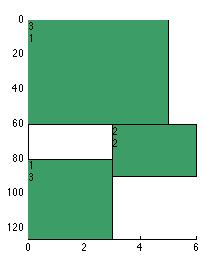
\includegraphics[width=.2\textwidth]{img/ph1}
	}
    \subfigure[Twee placeholders voor \textit{kortjes}]
    	{
			\label{fig:placeholders:ph2}
			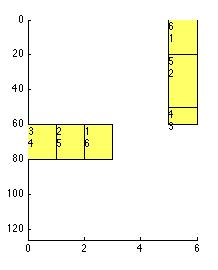
\includegraphics[width=.2\textwidth]{img/ph2}
	}
	\subfigure[Placeholder voor normale artikels]
    	{
			\label{fig:placeholders:ph3}
			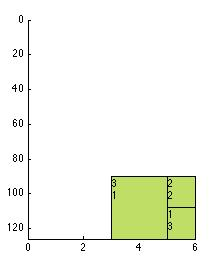
\includegraphics[width=.2\textwidth]{img/ph3}
	}
	\subfigure[Resultaat van inpassing placeholders (b) en (c) in (a)]
    	{
			\label{fig:placeholders:ph4}
			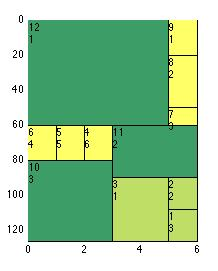
\includegraphics[width=.2\textwidth]{img/ph4}
	}
  \end{center}
  \caption{Het concept van placeholders}
  \label{fig:placeholders}
\end{figure}

De kracht van placeholders is tweeledig. Enerzijds is er bijna garantie dat een mooie paginalayout bekomen wordt (zonder chaotisch geplaaste rechthoeken). Elke rechthoek past immers perfect in een andere, grotere, rechthoek dewelke op zijn beurt ... . 

Anderzijds leent dit concept zich tot constraint programming. Het systeem bevat een reeks abstracte placeholders die in ��n keer of gedeeltelijk kunnen/moeten geconstrueerd worden. Bijvoorbeeld
\begin{itemize}
	\item 
		\begin{enumerate}
			\item
	Figuur \ref{fig:placeholders:ph1} (placeholder voor geschrankte pagina). In de eerste stap worden artikels 1 en 2 (vlnr, vbno) gezocht. De constraint op de rechthoek voor artikel 1 is bijvoorbeeld 
		\begin{eqnarray*}
			Article_{1}Width &\leq& PageWidth \\
			Article_{1}Height &\leq& PageHeight \label{eq:onderaan}
		\end{eqnarray*} 

De constraint op de rechthoek voor artikel 2 (geschrankt geplaatst: rechts uitgelijnd (eq. \ref{eq:rechts}) en onderaan tegen artikel 1 geplakt (eq. \ref{eq:onderaan})) is bijvoorbeeld 
		\begin{eqnarray}
			Article_{2}EndX &=& PageWidth \label{eq:rechts} \\
			Article_{2}StartY &=& Article_{1}EndY \label{eq:onderaan} \\
			Article_{1}Height + Article_{2}Height &\leq& PageHeight \label{eq:niethoger}
		\end{eqnarray} 
			
			\item
	Stap 1 is steeds dezelfde. Voor stap 2 zijn er 2 mogelijkheden: artikel 3 kan links naast artikel 2 liggen, of artikel 3 kan onder artikel 2 liggen. Over deze 2 mogelijkheden kan gebacktracked worden.
	
	\begin{itemize}
		\item \underline{Artikel 3 links naast artikel 2} (linksonder uitgelijnd (eq. \ref{eq:linksonder1} en \ref{eq:linksonder2}), tussen de rand en artikel 2 (eq. \ref{eq:randart2}), onder artikel 1 (eq. \ref{eq:onderart1}))
		
			\begin{eqnarray}
				Article_{3}StartX &=& 0 	\label{eq:linksonder1} \\
				Article_{3}EndY &=& PageHeight \label{eq:linksonder2} \\
				Article_{3}Width &\leq& Article_{2}StartX \label{eq:randart2} \\
				Article_{3}Height &\leq& Article_{1}EndY \label{eq:onderart1}
			\end{eqnarray}

		\item \underline{Artikel 3 onder artikel 2} (linksonder uitgelijnd (herbruik eq. \ref{eq:linksonder1} en \ref{eq:linksonder2}), onder artikel 2 (eq. \ref{eq:onderart2}))
		
			\begin{eqnarray}
				Article_{3}Height &\leq& Article_{2}EndY \label{eq:onderart2} \\
				Article_{3}Width &\leq& PageWidth \label{eq:randart2}
			\end{eqnarray}
	\end{itemize}
	
	Als artikel 3 geplaatst is, kunnen de overblijvende, lege rechthoeken (de witte rechthoeken van figuur \ref{fig:placeholders:ph1}) bepaald worden. Deze worden op hun beurt opgevuld met artikels of nieuwe placeholders.
	
	\item Figuur \ref{fig:placeholders:ph2} (placeholder verticale kolom voor $n$ kortjes). Deze kan in ��n stap opgezet worden en de constraints zijn eenvoudiger.
		\begin{eqnarray*}
			Article_{i}Width &=& 1 \\
			\sum_{i=1}^{n}{Article_{i}Height} &=& PlaceholderHeight
		\end{eqnarray*}
		
		Bij het zoeken naar artikels die in de placeholder passen kan bijvoorbeeld begonnen worden met $n=1$ (1 artikel met de hoogte van de placeholder). Indien dergelijk artikel niet bestaat, probeer voor $n=2$ (2 artikels die samen even hoog zijn als de placeholder), enzovoort.
\end{enumerate}
\end{itemize}

Zo kunnen verschillende structuren gedefinieerd worden.


\chapter{Relatie tussen stage en opleiding}
Het gestelde probleem is, in tegenstelling tot wat velen op het eerste zicht beweerden, niet triviaal. Er is kennis van zake nodig om abstract te kunnen redeneren, niet in termen van tekst (artikels) op paginas, maar van rechthoeken in andere rechthoeken tot rijen in matrices. De opleiding Ingenieurswetenschappen brengt daarvoor de juiste voorkennis en vaardigheden bij.

Het probleem moet compact genoeg kunnen voorgesteld worden (waar het Java schoentje waarschijnlijk wringt) om snel genoeg te kunnen zoeken in de verschillende mogelijkheden. Een ander facet is het efficient zoeken naar \textit{goede} oplossingen. Alle oplossingen overlopen duurt al minstens 5 dagen en volgens de schatting nog veel langer dan dat.

Een aantal vakken komen naar de voorgrond. Allereerst is er het vak `Artificiele Intelligentie'\footnote{H01O4A, D. De Schreye} waarin zoekmethodes aan bod komen (waaronder A*, Greedy Search en Branch and Bound). Het vak `Studie van Declaratieve Talen'\footnote{H04H5A, G. Janssens} introduceert Prolog en `Advanced Programming Lanugages for A.I.'\footnote{H02A8A, G. Janssens} vertelt iets meer over constraint programming en ECLiPSe.

De Prolog oplossing werd ge-embed in Java (een vereiste voor projecten die lopen bij XT-i). Het inlezen en parsen van XML bestanden komt in de opleiding niet aan bod, maar het concept XML wordt wel besproken in het vak `Gegevensbanken'\footnote{H01O9A, H. Olivi�}. Een goed OO-ontwerp maakt dat het Java programma eenvoudig en modulair is. Hiermee zijn de vakken `Objectgericht Programmeren'\footnote{H01P1A, E. Steegmans} en `Ontwerp en analyse van softwaresystemen, deel 1'\footnote{H04J9A, R. Wuyts} gerelateerd.

Hoewel niet gebruikt in deze oplossing is de achtergrondkennis over constraint programming (m.n. lineire programmas) in het vak `Besliskunde voor bedrijfsbeheer'\footnote{H01R7A, D. Cattrysse} relevant.

\chapter{Conclusie}
Een eerste opgave is het juist formuleren van het probleem. De oplossing zoals beschreven in algoritme 1 bleek onvoldoende schaalbaar te zijn. Een betere voorstelling is gegeven in algoritme 2. De variant met de insluitingsheuristiek levert beduidend betere oplossingen. In algoritme 2.1 zijn enkele extra constraints ge�mplementeerd. Er is convergentie merkbaar naar wat mensen een \textit{goede} layout zouden vinden en het soort layouts dat de bestaande (trage) oplossing produceert.

Hoewel misschien contradictorisch, geldt de regel: hoe meer constraints hoe beter. De zoekruimte wordt kleiner en zo komt men sneller tot een oplossing, hoe eerder een constraint faalt hoe eerder naar een volgende oplossing gezocht kan worden.

Hoewel niet alle constraints van de bestaande Java oplossing zijn overgenomen en de kwaliteit van de oplossingen misschien niet helemaal hetzelfde is, valt er toch iets te zeggen voor het verschil in uitvoeringstijd, nl. 2 uur tegenover 0,3 seconden.

Bij een volgende iteratie zou er toch gekeken moeten worden om het kern-zoekalgoritme van ECLiPSe tot een volwaardige component van het productiesysteem te verheffen.


\appendix

\chapter{Listings}
%	\section{Listings}

\begin{listing}
	\begin{verbatim}
	<all>
	  <pages>
	    <page id="5001" isleft="0" artikelslinks="false" margex="35.4325" 
	          margey="150.630644" usewidth="822.034" useheight="1132.025856"></page>
	    [...]
	    <page id="4995" isleft="1" artikelslinks="true" margex="35.4325" 
	          margey="73.8328262" usewidth="822.034" useheight="1208.8236738">
	      <ad id="5015" x="35.433" y="1208.957" width="266.452"  height="73.7"/>
	    </page>
	  </pages>
	\end{verbatim}
  \caption{Invoer XML bestand}
  \label{listing:inXML}
\end{listing}

\begin{listing}
	\begin{verbatim}
	  <artikels>
	    <artikel id="11490" type="Kopstuk" plaatsing="V">
	      <artlayout id="31075" width="683.139" height="529.0"/>
	      <artlayout id="31074" width="683.139" height="529.0"/>
	      [...]
	      <artlayout id="31073" width="544.243" height="625.0"/>
	    </artikel>
	    [...]
	    <artikel id="11509" type="Normaal" plaatsing="M">
	      <artlayout id="31057" width="405.348" height="319.0"/>
	      [...]
	      <artlayout id="31053" width="266.452" height="436.0"/>
	    </artikel>
	    [...]
	    <artikel id="11390" type="Kortje" plaatsing="A">
	      <artlayout id="30899" width="127.557" height="214.0"/>
	    </artikel>
	  </artikels>
	</all>
	\end{verbatim}
  \caption{Invoer XML bestand (vervolg)}
  \label{listing:inXML2}
\end{listing}

	%\section{Algoritme 1}
	
\begin{listing}
	\begin{verbatim}
		Page Size (WxH): [10, 15]
		Placing: artikel(id(11490), type(kopstuk), plaatsing(m), 
		   [layout(id(31073), width(7), height(9))])
		Placed: 31073 [1, 7, 1, 9]  % ([StartX, StartY, EndX, EndY])
		Placing: artikel(id(11387), type(normaal), plaatsing(v), 
		   [layout(id(31042), width(7), height(3))])
		Placed: 31042 [1, 7, 10, 12]
		Placing: artikel(id(11488), type(normaal), plaatsing(m), 
		   [layout(id(30945), width(4), height(3))])
		Placed: 30945 [1, 4, 13, 15]
		Placing: artikel(id(11391), type(kortje), plaatsing(a), 
		   [layout(id(31052), width(2), height(3))])
		Placed: 31052 [8, 9, 1, 3]
		Placing: artikel(id(11384), type(kortje), plaatsing(a), 
		   [layout(id(30902), width(2), height(3))])
		Placed: 30902 [8, 9, 4, 6]
	\end{verbatim}
  \caption{Algoritme 1: Opeenvolgende geplaatste artikels}
  \label{listing:opeenvolgendegeplaatsteartikels}
\end{listing}

\begin{listing}
	\begin{verbatim}
		 31073 31073 31073 31073 31073 31073 31073 31052 31052 .....
		 31073 31073 31073 31073 31073 31073 31073 31052 31052 .....
		 31073 31073 31073 31073 31073 31073 31073 31052 31052 .....
		 31073 31073 31073 31073 31073 31073 31073 30902 30902 .....
		 31073 31073 31073 31073 31073 31073 31073 30902 30902 .....
		 31073 31073 31073 31073 31073 31073 31073 30902 30902 .....
		 31073 31073 31073 31073 31073 31073 31073 ..... ..... .....
		 31073 31073 31073 31073 31073 31073 31073 ..... ..... .....
		 31073 31073 31073 31073 31073 31073 31073 ..... ..... .....
		 31042 31042 31042 31042 31042 31042 31042 ..... ..... .....
		 31042 31042 31042 31042 31042 31042 31042 ..... ..... .....
		 31042 31042 31042 31042 31042 31042 31042 ..... ..... .....
		 30945 30945 30945 30945 ..... ..... ..... ..... ..... .....
		 30945 30945 30945 30945 ..... ..... ..... ..... ..... .....
		 30945 30945 30945 30945 ..... ..... ..... ..... ..... .....
	\end{verbatim}
  \caption{Algoritme 1: Layout van de eerste oplossing}
  \label{listing:layouteersteopl}
\end{listing}

\begin{listing}
	\begin{verbatim}
		Placed: 30902 [9, 10, 4, 6]

		 31073 31073 31073 31073 31073 31073 31073 31052 31052 .....
		 31073 31073 31073 31073 31073 31073 31073 31052 31052 .....
		 31073 31073 31073 31073 31073 31073 31073 31052 31052 .....
		 31073 31073 31073 31073 31073 31073 31073 ..... 30902 30902
		 31073 31073 31073 31073 31073 31073 31073 ..... 30902 30902
		 31073 31073 31073 31073 31073 31073 31073 ..... 30902 30902
		 31073 31073 31073 31073 31073 31073 31073 ..... ..... .....
		 31073 31073 31073 31073 31073 31073 31073 ..... ..... .....
		 31073 31073 31073 31073 31073 31073 31073 ..... ..... .....
		 31042 31042 31042 31042 31042 31042 31042 ..... ..... .....
		 31042 31042 31042 31042 31042 31042 31042 ..... ..... .....
		 31042 31042 31042 31042 31042 31042 31042 ..... ..... .....
		 30945 30945 30945 30945 ..... ..... ..... ..... ..... .....
		 30945 30945 30945 30945 ..... ..... ..... ..... ..... .....
		 30945 30945 30945 30945 ..... ..... ..... ..... ..... .....
	\end{verbatim}
  \caption{Algoritme 1: Layout van de volgende oplossing (bemerk verplaatst artikel 30902)}
  \label{listing:volgendeopl}
\end{listing}

	%\paragraph{Algoritme 2}
\begin{listing}
	\begin{verbatim}
Trying Article: article(11490, kopstuk, m, [layout(31075, 683, 529), ...
 Trying Page   : page(5001, 0.0, 822, 1132, [anchor(0, 0), anchor(0, 1132), ...
  Trying Layout : layout(31075, 683, 529)
   Trying Anchor : anchor(0, 0)
    DownRight     : [0, 683, 0, 529]
    Score          : 4373.60306827909
Found a solution with cost -4373.60306827909
   Trying Anchor : anchor(0, 1132)
   Trying Anchor : anchor(822, 0)
    DownLeft      : [139, 822, 0, 529]
    Score          : 4373.60306827909
   Trying Anchor : anchor(822, 1132)
  Trying Layout : layout(31074, 683, 529)
   Trying Anchor : anchor(0, 0)
    DownRight     : [0, 683, 0, 529]
    Score          : 4373.60306827909
   Trying Anchor : anchor(0, 1132)
   Trying Anchor : anchor(822, 0)
    DownLeft      : [139, 822, 0, 529]
    Score          : 4373.60306827909
   Trying Anchor : anchor(822, 1132)
  Trying Layout : layout(31072, 683, 529)

[...]	

Found no solution with cost -1.0Inf .. -4374.60306827909
****** Allocation of Article ******
Article    : article(11490, kopstuk, m, [layout(31075, 683, 529), ...
Allocation : [anchor(0, 0), allocation(5001, 11490, 31075, 0, 0, 683, 529) ...
Score      : 4373.60306827909
Result     : [page(5001, 0.0, 822, 1132, [anchor(0, 0), anchor(0, 529), ...
Remaining  : [article(11491, kopstuk, m, [layout(30927, 683, 489), ...

[... ...]

Found no solution with cost -1.0Inf .. 1.0Inf
***** Failed to place 25 articles *****
Remaining  : [article(11383, kopstuk, m, [layout(30931, 683, 443), ...
	\end{verbatim}
  \caption{Algoritme 2: Uitvoer}
  \label{listing:uitvoeralg2}
\end{listing}

\begin{figure}[h]
  \begin{center}
    \subfigure[Eerste oplossing met Greedy variant]
    	{
			\label{fig:layouts:greedy}
			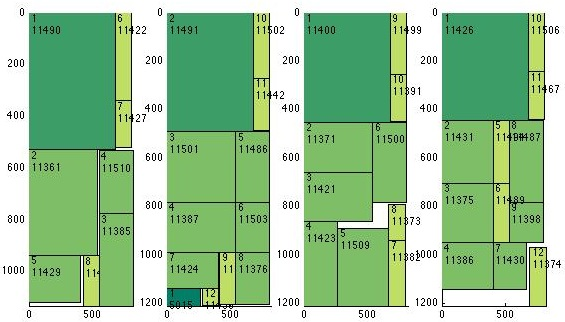
\includegraphics[width=\textwidth]{img/bestfirst}
		}
    \subfigure[Eerste oplossing met Complete variant]
    	{
			\label{fig:layouts:complete}
			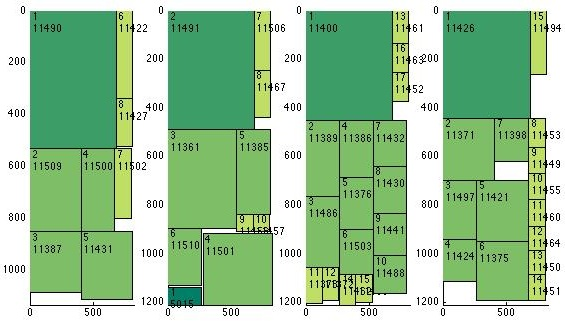
\includegraphics[width=\textwidth]{img/complete1}
		}
  \end{center}
  \caption{Eerste layouts gegenereerd met de verschillende zoekmethodes}
  \label{fig:layouts}
\end{figure}

\begin{listing}
	\begin{verbatim}
<pages>
  <page id="5001" ...
  <page id="4995" ...>
      <ad height="73.7" id="5015" width="266.452" x="35.433" y="1208.957"/>
  </page>
  <page id="4997" ...
  <page id="4999" ...
</pages>
<artikels>
  <artikel id="11490" layoutid="31075" pageid="5001" startx="0" starty="0"
  	  plaatsing="M" type="Kopstuk">
    <artlayout height="529.0" id="31075" width="683.139"/>
    <artlayout height="529.0" id="31074" width="683.139"/>
    <artlayout height="529.0" id="31072" width="683.139"/>
    <artlayout height="625.0" id="31073" width="544.243"/>

[...]
	\end{verbatim}
  \caption{Resultaat in XML, bemerk de toevoeging van layoutId, startX en startY.}
  \label{listing:uitvoerxml}
\end{listing}

\end{document}